\section[Le architetture]{Le architetture}
\label{sec:architectures}
\sectionframe{images/covers/cover_architecture.jpeg}{Le architetture}	


\subsection[I componenti essenziali]{I componenti essenziali}
\begin{frame}
	\frametitle{I componenti essenziali}
	
	\begin{block}{I componenti essenziali}
		Abbiamo chiarito quali sono i principali \textit{componenti elettronici} utilizzati in un computer e più nello specifico nei suoi componenti.\\~\\
		Definiamo brevemente quali sono i \textbf{componenti essenziali} che costituiscono un computer:
		\begin{itemize}
			\item \textit{il processore}
			\item \textit{la memoria}
			\item \textit{l'input/output (I/O)}
			\item \textit{il BUS}
		\end{itemize}
		
	\end{block}
	
\end{frame}



%\begin{frame}
%	\frametitle{L'architettura di un computer}
%	
%	\begin{block}{L'architettura di un computer}
%		In generale, l'architettura di un computer può essere divisa in tre parti principali:
%		\begin{itemize}
%			\item il processore
%			\item la memoria
%			\item l'input/output (I/O)
%		\end{itemize}
%	\end{block}
%	
%%	\begin{figure}[!htbp]
%%		\centering 
%%		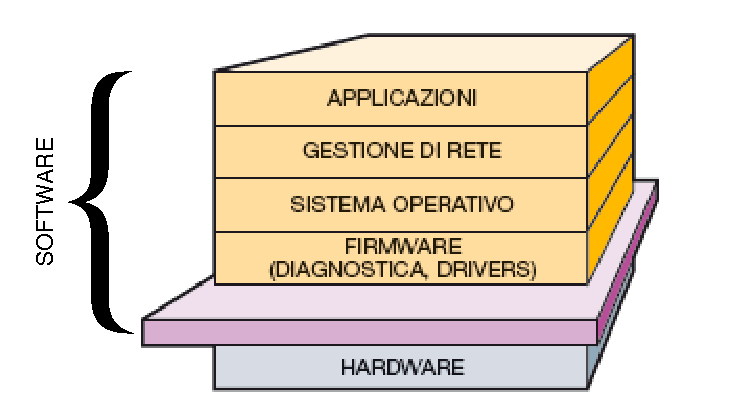
\includegraphics[width=0.6\linewidth]{images/3_architetture/hd-sw.pdf}
%%%			\caption{}
%%	\end{figure}
%	
%\end{frame}


\subsubsection[Il processore]{Il processore}
\begin{frame}
%	\frametitle{L'architettura di un computer}
	
	\begin{block}{Il processore}
		Il \textbf{processore}, noto anche come "microprocessore", è il "cervello" del computer, ed è responsabile dell'esecuzione delle istruzioni contenute nel software.
	\end{block}

	\begin{columns}			
		\column{0.5\linewidth}
		\begin{figure}[!htbp] 
			\centering
			%\advance\leftskip-0.25cm
			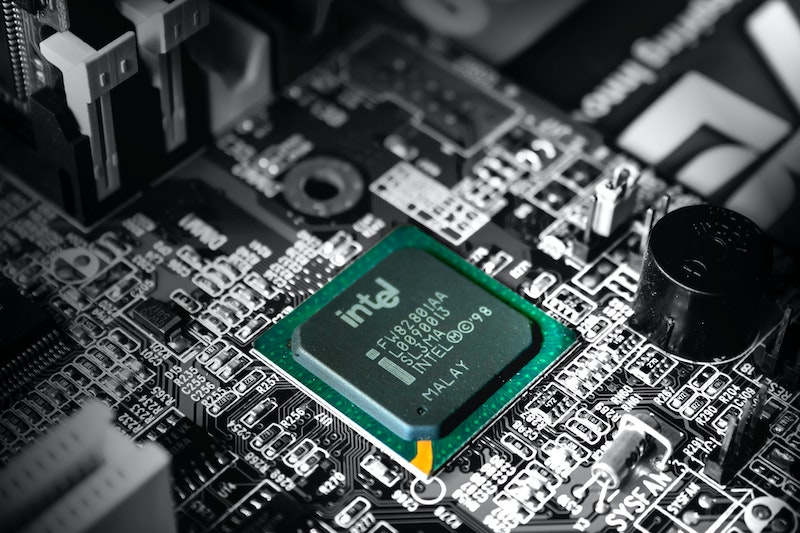
\includegraphics[width=1.0\linewidth]{images/3_architetture/intel.jpg}
			\caption{Processore Intel}
			\label{fig:architectures_intel}
		\end{figure}
					
		\column{0.5\linewidth}
		\begin{figure}[!htbp] 
			\centering
			%\advance\leftskip-0.25cm
			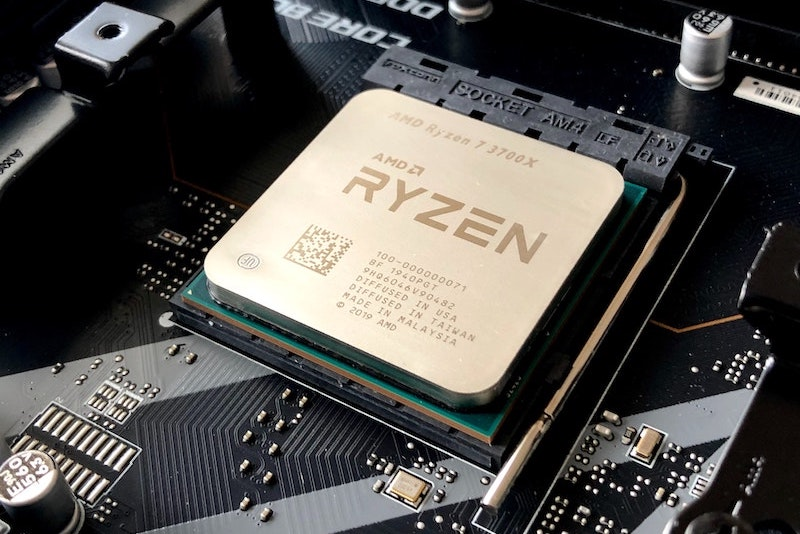
\includegraphics[width=1.0\linewidth]{images/3_architetture/ryzen.jpg}
			\caption{Processore AMD Ryzen}
			\label{fig:architectures_ryzen}
		\end{figure}
		
	\end{columns}
	
\end{frame}



\subsubsection[La memoria]{La memoria}
\begin{frame}
%	\frametitle{L'architettura di un computer}
	
	\begin{block}{La memoria}
		La \textbf{memoria} è dove vengono archiviati i dati e le istruzioni che vengono utilizzati dal processore. Possiamo distinguere due tipi di memoria:
		\begin{itemize}
			\item \textbf{memoria principale}, utilizzata per archiviare i dati su cui il processore sta attualmente lavorando.
			In questa categoria la memoria più importante è la memoria \underline{RAM} (anche detta memoria centrale).
			%Può essere classificata come memoria principale anche la \underline{ROM} (Read Only Memory), che è una memoria persistente a sola lettura.
			\item \textbf{memoria secondaria}, come il \underline{disco rigido} o il \underline{solid state drive}, che vengono utilizzati per archiviare i dati a lungo termine.
		\end{itemize}
%		\begin{itemize}
%			\item la \textbf{memoria RAM} (Random Access Memory), che viene utilizzata per archiviare i dati che il processore sta attualmente lavorando
%			\item la \textbf{memoria di massa}, come il disco rigido o il solid state drive, che viene utilizzata per archiviare i dati a lungo termine.
%		\end{itemize}
	\end{block}
	
	\begin{columns}			
		\column{0.5\linewidth}
		\begin{figure}[!htbp]
			\centering
			%\advance\leftskip-0.25cm
			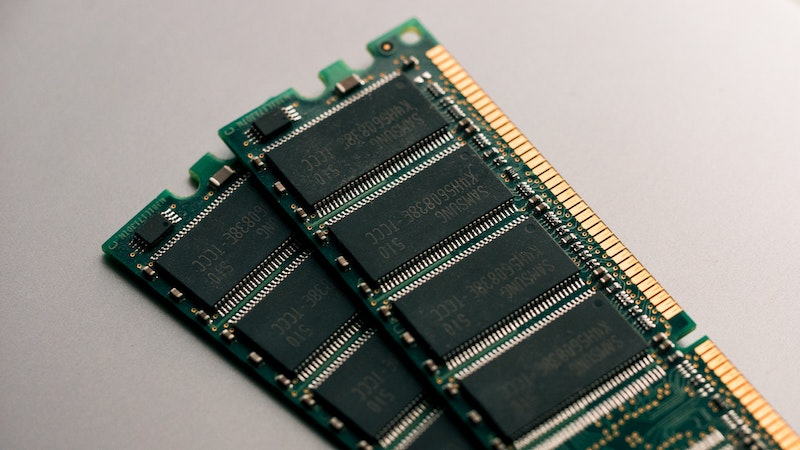
\includegraphics[width=0.78\linewidth]{images/3_architetture/memory_ram.jpg}
			\caption{RAM (Random Access Memory)}
			\label{fig:architectures_memory_ram}
		\end{figure}
					
		\column{0.5\linewidth}
		\begin{figure}[!htbp] 
			\centering
			%\advance\leftskip-0.25cm
			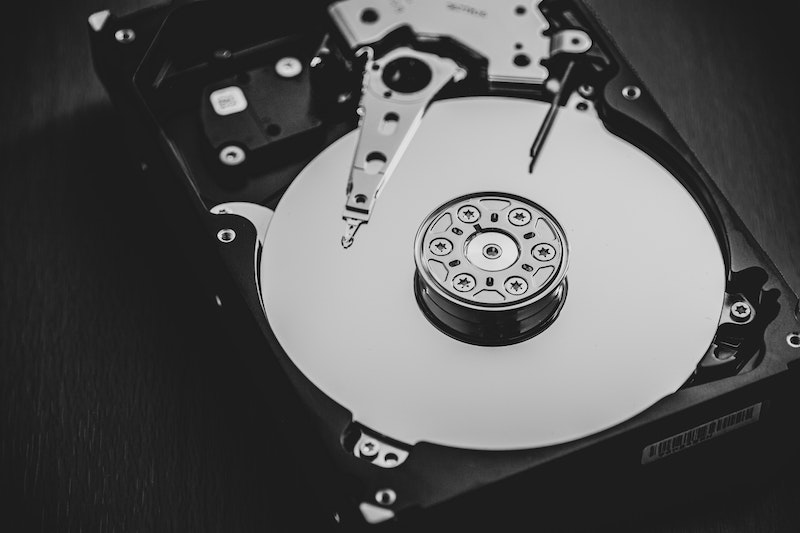
\includegraphics[width=0.68\linewidth]{images/3_architetture/memory_hdd.jpg}
			\caption{L'interno di un Hard Disk}
			\label{fig:architectures_memory_hdd}
		\end{figure}
		
	\end{columns}
	
\end{frame}


\subsubsection[L'input/output (I/O)]{L'input/output (I/O)}
\begin{frame}
%	\frametitle{L'architettura di un computer}
	
	\begin{block}{L'input/output (I/O)} 
		L'\textbf{input/output} (I/O) gestisce il flusso di dati tra il computer e l'esterno, attraverso dispositivi come il monitor, la tastiera e il mouse.
	\end{block}
	
	\begin{figure}[!htbp] 
		\centering
		%\advance\leftskip-0.25cm
		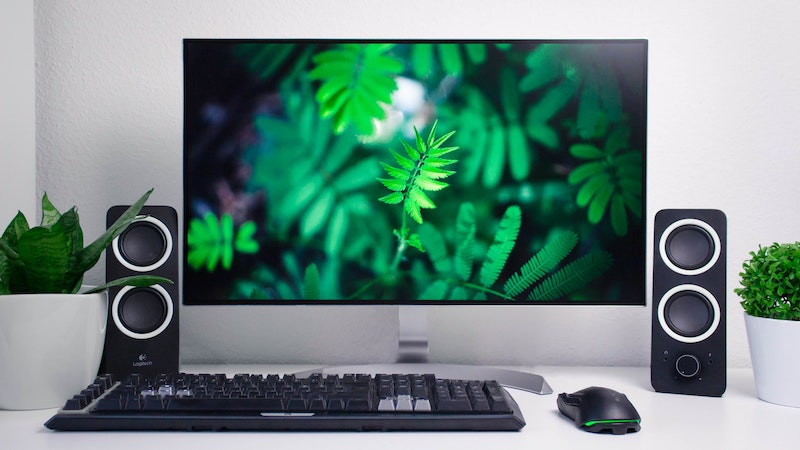
\includegraphics[width=0.8\linewidth]{images/3_architetture/io.jpg}
		\caption{Monitor, tastiera, mouse e casse}
		\label{fig:architectures_io}
	\end{figure}
	 
\end{frame}


\subsubsection[Il BUS]{Il BUS}
\begin{frame}
%	\frametitle{L'architettura di un computer}
	
	\begin{block}{Il BUS} 
		Il \textbf{BUS} è il canale di comunicazione che permette di collegare tra loro i componenti dell’architettura, consentendo il transito delle informazioni.\\
		Possiamo paragonare i BUS a delle \textbf{autostrade per i bit}.\\
		Distinguiamo tre diverse linee (che approfondiremo in seguito):
		\begin{itemize}
			\item \textit{Control BUS} (BUS di controllo)
			\item \textit{Address BUS} (BUS degli indirizzi)
			\item \textit{Data BUS} (BUS dati)
		\end{itemize}

	\end{block}
	
	\begin{figure}[!htbp] 
		\centering
		%\advance\leftskip-0.25cm
		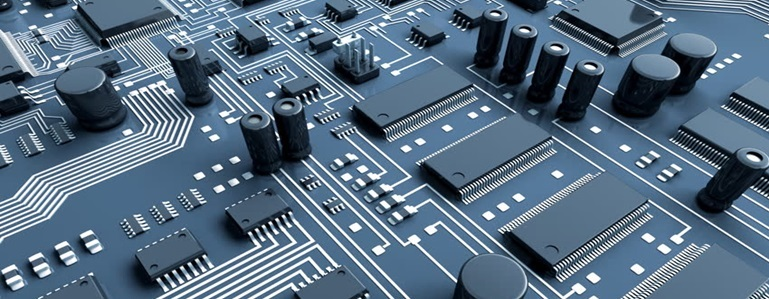
\includegraphics[width=0.75\linewidth]{images/3_architetture/bus.jpg}
%		\caption{}
%		\label{fig:architectures_bus} 
	\end{figure}
	 
\end{frame}


\begin{frame}
%	\frametitle{L'architettura di un computer}
	
	\begin{block}{Altre componenti}
		Altre componenti comuni di un computer possono includere schede di espansione, che forniscono ulteriori funzionalità al computer, come ad esempio la possibilità di collegare dispositivi esterni o di aggiungere ulteriori porte di I/O.
	\end{block}
	
	
	
	\begin{columns}			
		\column{0.4\linewidth}
		\begin{figure}[!htbp]
			\centering 
			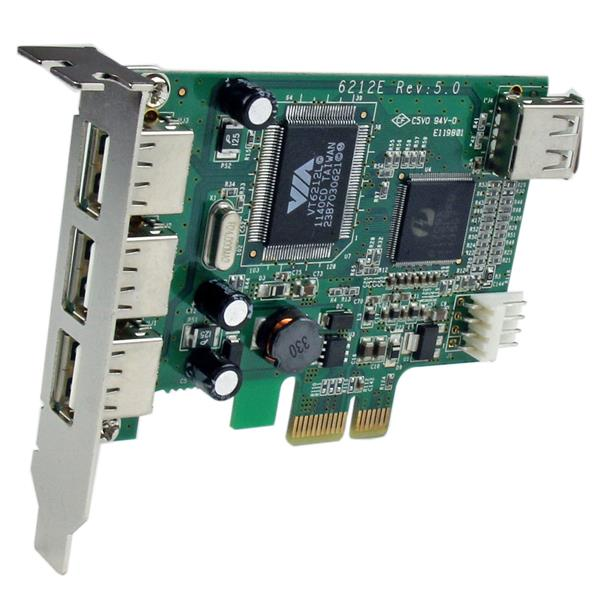
\includegraphics[width=0.82\linewidth]{images/3_architetture/pcie_2.jpg}
			\caption{PCI Express x1}
		\end{figure}
		
		\column{0.6\linewidth}
		\begin{figure}[!htbp]
			\centering 
			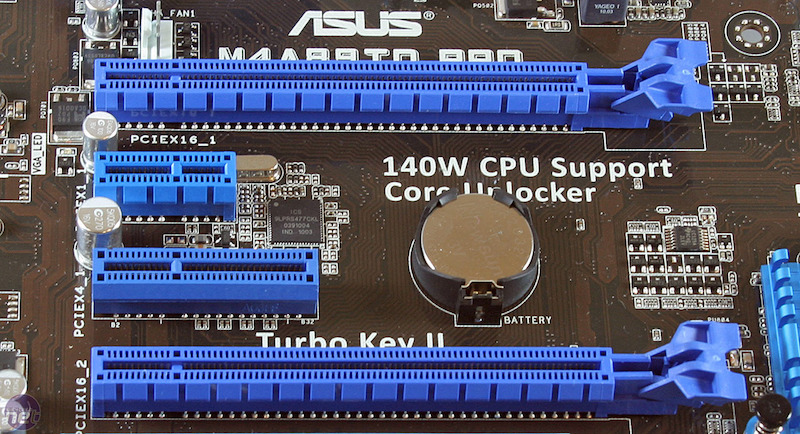
\includegraphics[width=1.0\linewidth]{images/3_architetture/pcie_1.jpg}
			\caption{PCI Express: x16, x1, x4, x16}
		\end{figure}
	\end{columns}
	
\end{frame}


\subsection[Le architetture / I modelli]{Le architetture / I modelli}
\begin{frame}
	\frametitle{Le architetture / I modelli}
	
%	\begin{block}{Le architetture / I modelli}
	
		In ingegneria informatica, l'\underline{\textbf{architettura}} di un computer è una descrizione della struttura di un sistema informatico formato da componenti.
		\begin{itemize}
			\item Ad un alto livello può essere intesa come una \textbf{descrizione che ignora i dettagli dell'implementazione} (\underline{\textbf{come nei modelli}}).
			\item Ad un livello più dettagliato, la descrizione può includere: il design dell'architettura dell'insieme di istruzioni, il design della microarchitettura, il design logico e l'implementazione.
		\end{itemize}
		~\\
		\pause
		Le due architetture maggiormente utilizzate per illustrare il funzionamento di massima di un computer sono:
		\begin{itemize}
			\item l'\textbf{architettura von Neumann} (aka \textit{modello di von Neumann} o \textit{architettura Princeton})
			\item l'\textbf{architettura Harvard} (aka \textit{modello di Harvard})
		\end{itemize}
%	\end{block}
	
\end{frame}

\subsubsection[L'architettura von Neumann]{L'architettura von Neumann}
\begin{frame}
	\frametitle{L'architettura von Neumann}
	
	
	\begin{columns}			
		\column{0.75\linewidth}
		\begin{block}{L'architettura von Neumann}
			Si tratta di uno schema a blocchi che illustra il modello di funzionamento di massima di un computer, ideato dal ricercatore ungherese \textbf{Janus Neumann}, naturalizzato americano (John von Neumann). Il modello è stato ideato per la prima volta durante la progettazione del primo computer elettronico, chiamato IAS machine presso l’Institute for Advanced Study, a \textbf{Princeton} negli Stati Uniti tra il 1945 e il 1951.\\~\\
			
			L'architettura von Neumann descrive il comportamento di una macchina che il suo inventore chiamò \underline{\textbf{stored-program computer}}.
		\end{block}
		
		\column{0.25\linewidth}
		\begin{figure}[!htbp]
			\centering 
			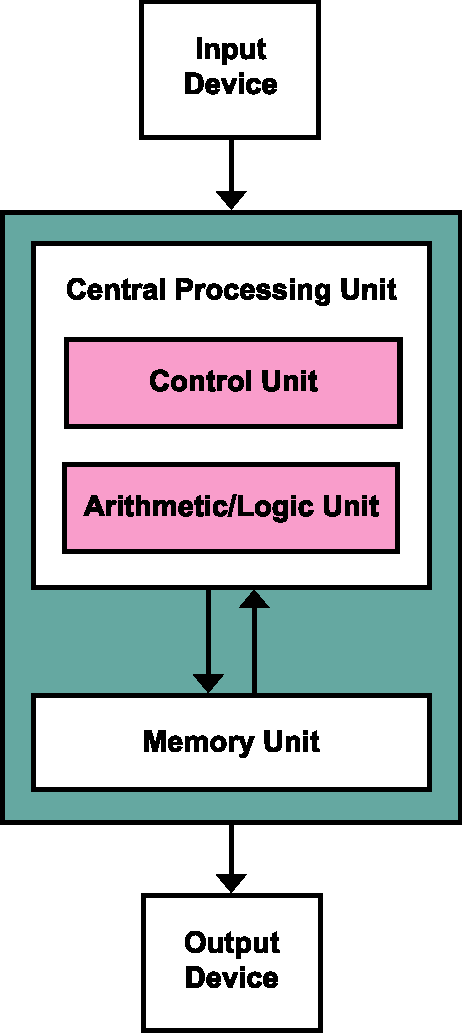
\includegraphics[width=0.90\linewidth]{images/3_architetture/architecture_von_neumann.pdf}
%			\caption{} 
		\end{figure}
	\end{columns}
	
	
\end{frame}


\begin{frame}
	\frametitle{L'architettura von Neumann}
	
	
	\begin{columns}			
		\column{0.75\linewidth}
		\begin{block}{Stored-program computer}
			\begin{itemize}
				\item \textbf{Computer}: 
					rappresenta la CPU che compie azioni di elaborazione come, prelevare o modificare il contenuto della memoria o informazioni dai dispositivi di input/output.\\
					La CPU è in grado di eseguire le proprie azioni in modo sequenziale.
				\item \textbf{Stored-program}: indica che le istruzioni che la CPU deve eseguire sono collocate (stored) nella memoria del computer e l'insieme delle istruzioni rappresenta il programma (program) che deve essere eseguito.\\
					\underline{\textbf{Nella memoria}} risiedono, oltre alle \underline{\textbf{istruzioni}} anche i \underline{\textbf{dati}} sui quali tali programmi operano.
			\end{itemize}
		\end{block}
		
		\column{0.25\linewidth}
		\begin{figure}[!htbp]
			\centering 
			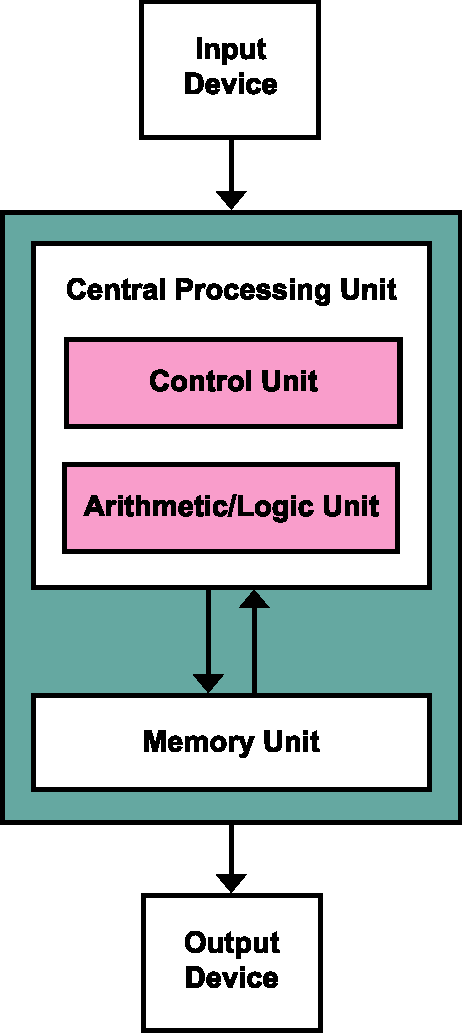
\includegraphics[width=0.90\linewidth]{images/3_architetture/architecture_von_neumann.pdf}
%			\caption{} 
		\end{figure}
	\end{columns}
	
	
\end{frame}


\begin{frame}
	\frametitle{L'architettura von Neumann}
	
	\begin{figure}[!htbp]
		\centering 
		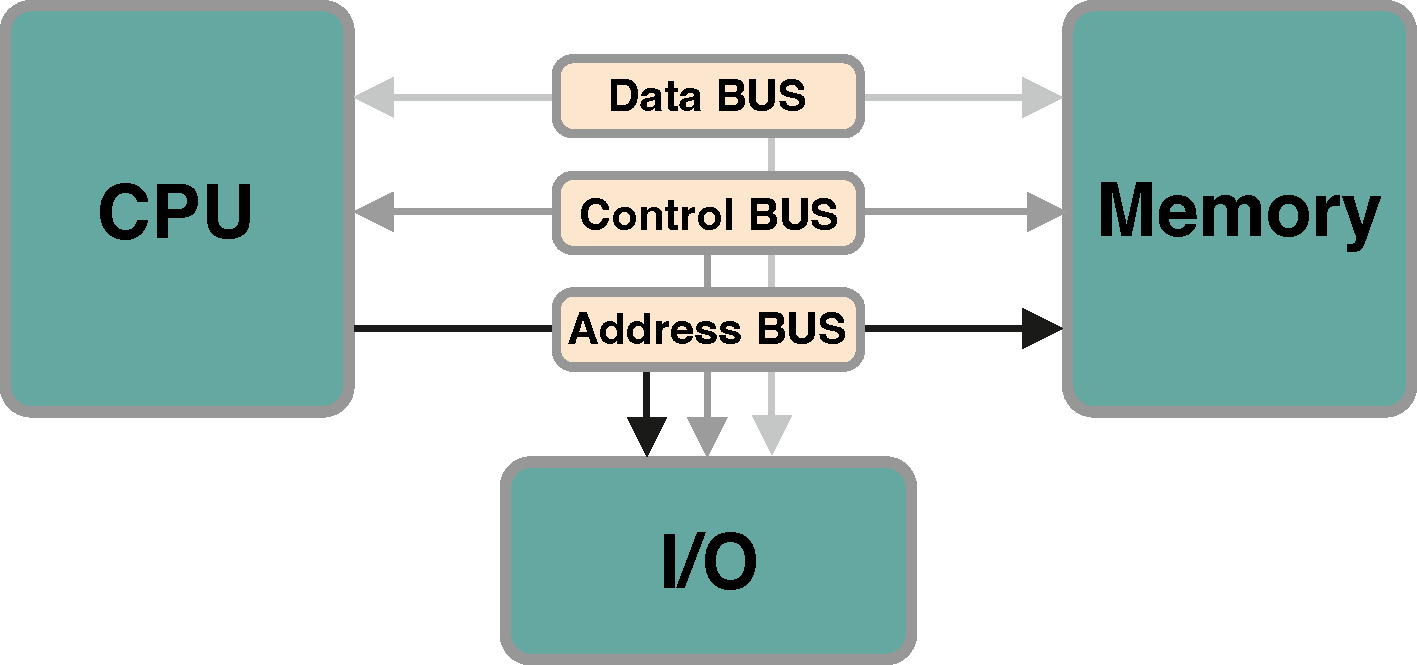
\includegraphics[width=0.9\linewidth]{images/3_architetture/architecture_von_neumann_system_bus.pdf}
			\caption{Schema dell'architettura System bus, evoluzione di quella di von Neumann} 
	\end{figure}
	
\end{frame}





\subsubsection[L'architettura Harvard]{L'architettura Harvard}

\begin{frame}
	\frametitle{L'architettura Harvard}
	
	\begin{block}{L'architettura Harvard}
		A differenza dell'architettura di von Neumann nel quale i dati e le istruzioni condividono la stessa memoria, l'\textbf{architettura di Harvard} dedica \underline{\textbf{due memorie distinte per i dati e per le istruzioni}}.\\
		Si tratta di una soluzione \textbf{più efficiente e ottimizzata}, ma tuttavia molto \textbf{più costosa}.\\~\\
		L'architettura Harvard è un modello applicato alla progettazione di 	\textit{processori specializzati} come i DSP (Digital Signal Processor) che vengono utilizzati per il trattamento dei dati audio o video. Inoltre molti \textit{microcontrollori} impiegati in applicazioni industriali utilizzano questa architettura.
	\end{block}
	
	
\end{frame}


\begin{frame}
	\frametitle{L'architettura Harvard}
	
	\begin{figure}[!htbp]
		\centering 
		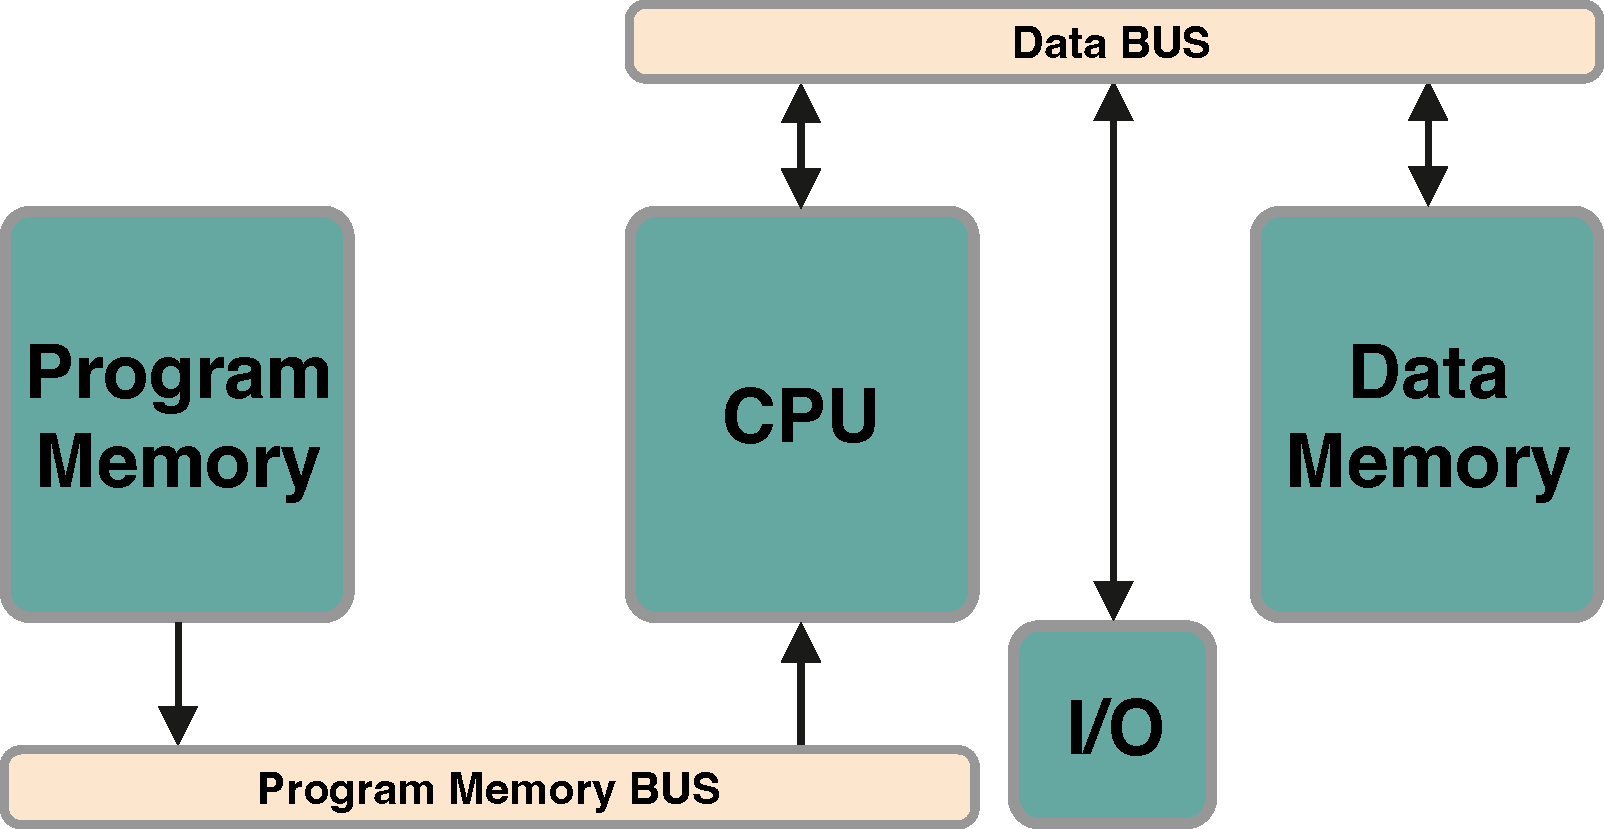
\includegraphics[width=0.9\linewidth]{images/3_architetture/architecture_harvard.pdf}
			\caption{Struttura dell'architettura Harvard} 
	\end{figure}
	
\end{frame}
